\documentclass[utf8,english]{psta}% 
% look at psta-man.tex, please!
% Refine, please, UDC and MSC Classification indexеs for Your paper
\subjclass[UDC]{519.68}
\subjclass[BBC]{32.973.202-018.2}
\subjclass[2010]{97P30; 97P20, 97R40}

% data in Russian comes inside the Russian section(s) which is already here
%\selectlanguage{russian}
%\title{Векторизация римановского решателя с использованием набора инструкций AVX-512}
% Last name, coma other names 
%\author{Рыбаков, Алексей}
% Organisation, where the work done
%\address{Joint Supercomputer Center of the Russian Academy of Sciences -- branch of Scientific Research Institute of System Analysis of the Russian Academy of Sciences (JSCC RAS -- branch of SRISA), 119334, Moscow, Leninsky prospect, 32a.}
% author email
%\email{rybakov@jscc.ru}

% Last name, coma other names 
%\author{Шумилин, Сергей}
% Organisation, where the work done
%\address{Joint Supercomputer Center of the Russian Academy of Sciences -- branch of Scientific Research Institute of System Analysis of the Russian Academy of Sciences (JSCC RAS -- branch of SRISA), 119334, Moscow, Leninsky prospect, 32a.}
% author email
%\email{shumilin@jscc.ru}

% Two lines of key words
%\keywords{}
%\begin{abstract} 
%Численные методы, базирующиеся на решении задачи Римана о распаде произвольного разрыва, крайне требовательны к вычислительным ресурсам.
%Для применения данных численных методов на современных расчетных сетках требуется использование суперкомпьютера.
%Среди различных инструментов повышения производительности суперкомпьютерных приложений можно выделить векторизацию программного кода.
%Набор инструкций AVX-512 обладает рядом уникальных возможностей, позволяющих применить векторизацию к программному контексту римановского решателя, что ведет значительному ускорению решателя.
%\end{abstract}

\selectlanguage{english}
% All the same in English 
\title[vectorization of the Riemann solver]{Vectorization of the Riemann solver using the AVX-512 instruction set}
% Last name, coma other names 
\author{Rybakov, Alexey}
% Organisation, where the work done
\address{Joint Supercomputer Center of the Russian Academy of Sciences -- branch of Scientific Research Institute of System Analysis of the Russian Academy of Sciences (JSCC RAS -- branch of SRISA), 119334, Moscow, Leninsky prospect, 32a.}
% author email
\email{rybakov@jscc.ru}
% support notes
%\thanks{TODO}
% Other information about author only on paper language 
\info{Rybakov Alexey Anatolyevich - candidate of Physico-Mathematical Sciences, leader researcher of JSCC RAS - Branch of the Federal State Institution NIISI RAS. Research interests include mathematical modelling of gas dynamics problems using supercomputers, methods for constructing and managing computational grids, discrete mathematics, graph theory, random graph models, parallel programming, and functional programming.}
\image{pics/rybakov}
\orcid{0000-0002-9755-8830}  

% Last name, coma other names 
\author{Shumilin, Sergey}
% Organisation, where the work done
\address{Joint Supercomputer Center of the Russian Academy of Sciences -- branch of Scientific Research Institute of System Analysis of the Russian Academy of Sciences (JSCC RAS -- branch of SRISA), 119334, Moscow, Leninsky prospect, 32a.}
% author email
\email{shumilin@jscc.ru}
\info{Shumilin Sergey Sergeevich - senior engineer of JSCC RAS - Branch of the Federal State Institution NIISI RAS. Areas of scientific interest are machine learning, data analysis, algorithms, parallel programming.}
\image{pics/shumilin}
\orcid{0000-0002-3953-7054} 

\keywords{Riemann problem of the decay of an arbitrary discontinuity, Riemann solver, AVX-512, KNL, vectorization, intrinsic functions}
\begin{abstract} 
Numerical methods based on solving the Riemann problem of the decay of an arbitrary discontinuity are extremely demanding of computational resources.
Applying the data of numerical methods to modern computational grids requires the use of a supercomputer.
Among the various tools for improving the performance of supercomputer applications, we can emphasize the vectorization of program code.
The AVX-512 instruction set has a number of unique features allowing to apply vectorization to the Riemann solver software context, which results in a significant acceleration of the solver.
Using the exact Riemann solver as an example, the article discusses practical approach to vectorizing a various program contexts, including simple linear blocks, regions with complex control, and nested loops.
The basis of the approach under consideration is the possibility of simultaneously executing several instances of some pure function on the same processor core.
This feature is achieved by translating the program code into the predicate form and using AVX-512 vector instructions.
In this case the number of simultaneously running instances is equal to the width of the vector.
It is shown that using the features of the AVX-512 instruction set allows to successfully vectorize the considered program context.
The proposed approach can be applied to vectorize a wide range of applications.
\end{abstract}

\begin{document}          
\maketitle 
\section*{Introduction}
The solution of the Riemann problem is used in numerical methods for non-stationary problems with large discontinuities \cite{KulPogSemRiemann}.
At the same time, this approach can be applied both to ordinary single-component gas-dynamic equations and to the equations of multicomponent gas dynamics \cite{BorRykRiemann}.
The Godunov method for solving systems of unsteady equations of gas dynamics \cite{Godunov} is based on an exact or approximate solution of the Riemann problem.
In this method, at each iteration of the calculations, the Riemann problem is solved on each face of each cell of the computational grid to determine the flows through these faces.
Due to the fact that the sizes of computational grids, which are used today for carrying out calculations, amount to tens, hundreds of millions of cells and more, it is necessary to use supercomputers and the entire spectrum of approaches to parallel computing.
To increase the efficiency of supercomputer computing, tools such as MPI, OpenMP, OpenACC and others are used.

The most low-level approach used to improve the performance of supercomputer applications is code vectorization.
The use of a special instruction set AVX-512 has unique features that make it possible to create an effective parallel code, which leads to a multiple acceleration of supercomputer applications.

Improving the performance of Riemann solvers on parallel architectures has been the subject of much research, which continues to this day, as new architectures constantly emerge with new features.
The \cite{Shumlak} demonstrated an algorithm for parallelizing numerical methods using an approximate Riemann solver for problems of magnetohydrodynamics, leading to parallel operation on a multiprocessor machine with parallelization efficiency close to unity.
The work \cite{Schive} provides a comprehensive study on the parallelization of computational methods based on the Riemann solver using MPI, OpenMP and graphics accelerators.
As a result, good performance in terms of scalability was demonstrated, in particular, a strong scalability indicator at around 85\%.
The \cite{Mandli} work highlights the use of the PetClaw tool, which allows to apply numerical methods based on the Riemann solver on several thousand computational processes with a parallelization efficiency close to unity.
The works \cite{Kulikov}, \cite{Kulikov2} highlighted the issues of parallel implementation of the AstroPhi program for modeling astrophysical flows.
It is shown that the current implementation allows achieving almost 50\% of the scalar peak performance of the Intel Xeon Phi KNC coprocessors and provides the estimate of the expected effect of future vectorization (more than 80\% of the total peak performance).
As one of the most detailed studies on the vectorization of Riemann solvers, we can mention the work \cite{BaderSWEVect}, which deals with the optimization of an approximate Riemann solver for solving shallow water equations.
The approaches used made it possible to achieve acceleration of 6-7 times on the Intel Xeon Phi KNC coprocessors on real operations with single precision.
Later this study was continued and the work \cite{FerreiraSWEVect} describes methods by which acceleration was obtained in the 2.4-6.5 times range for double precision operations (calculations were performed on Intel Xeon Phi KNL microprocessors).

This article discusses the vectorization of the exact Riemann solver containing complex structures, including solving a nonlinear equation and complex control.
The article shows that using the features of the AVX-512 instruction set allows you to successfully vectorize this software context.

The main contribution of this article is the development of approaches to vectorization of complex program context using a unique set of instructions AVX-512.
The exact Riemann solver is very suitable for this purpose, as it has a compact implementation and at the same time contains a number of features of the program context that require their own techniques during vectorization.

The first section of the article provides a brief description of the features of the AVX-512 instruction set, which allow vectorization of a complex program context using a predicate code representation.
The second section presents the general scheme of the exact Riemann solver, and sections 3-5 reveal the features of the vectorization of its individual parts (simple linear context, sections with complex controls and a nested loop).
Section 6 presents the results of numerical experiments on the Intel Xeon Phi KNL microprocessor, and section 7 presents a comparison with related works.

\section{Features of the AVX-512 instruction set}

The AVX-512 instruction set is an extension of the 256-bit AVX instruction of the Intel x86 architecture.
This instruction set is supported in the second-generation Intel Xeon Phi microprocessor (Knight Landing, KNL) and Intel Xeon Skylake families.

AVX-512 instructions work with 512-bit vector registers (\texttt{zmm}), which may contain integer or real data.
Each \texttt{zmm} register is capable of holding, for example, 8 real double precision values (\texttt{double}) or 16 real single precision values (\texttt{float}).
The AVX-512 instruction set implements a variety of operations with vector arguments, including arithmetic operations, comparison operations, memory read and write operations, transcendental operations, combined operations like $\pm a \cdot b \pm c$, elements permutation operations vectors and others.

To support selectively applying packed data operations to specific vector elements, most of the AVX-512 instructions use special mask registers as arguments.
There are 8 such registers (\texttt{k0-k7}).
When performing a vector operation, the element of the result vector will be calculated only if the bit of the mask with the corresponding number is set to one, otherwise the operation for these elements will be ignored.
This unique feature of the AVX-512 instruction set provides the implementation of the predicate execution mode \cite{VolOkuPred}, which is supported in such architectures as ARM or <<Elbrus>> \cite{KimElbrus}.
The presence of the predicate execution mode allows you to apply merger optimization of execution branches and, thus, get rid of unnecessary control transfer operations, which helps to create highly efficient parallel code.

Other important features of the AVX-512 instruction set include multiple reads of vector elements located in memory with arbitrary offsets from the base address, as well as similar operations of writing vector elements into memory with arbitrary offsets (\texttt{gather/scatter} operations).
Although these operations are extremely slow, they in some cases help to significantly simplify the logic of vectorized code.
It should also be noted a large variety of different operations of permutation, mixing, duplication, transfer of vector elements, which allows arbitrary change the order of data processing.
Also, combined operations that combine the multiplication and addition operations into one operation can bring significant acceleration.

To simplify the use of vector instructions for optimizing the program code for the icc compiler, special intrinsic functions have been developed (they are defined in the header file \texttt{immintrin.h}) \cite{IntelIntrGuide}.
These functions do not cover the entire set of AVX-512 instructions, however they eliminate the need to manually write assembly code.
Instead, it is possible to operate the built-in data types for 512-bit vectors and use them when working with the intrinsics functions as normal base types (the \texttt{zmm} registers will be used when building the executable code by the compiler).
Some intrinsic functions correspond not to one separate command, but to an entire sequence, such as the group of \texttt{reduce} functions, while others simply expand into a call of library function (for example, trigonometric functions or the \texttt{hypot} function).

In this article, we consider the features of the Riemann solver in the classical implementation of E.~F.~Toro \cite{TorRiemann} and describe approaches that allow to vectorize this solver to simultaneously solve 16 copies of the Riemann problem of decay of an arbitrary discontinuity at once.

\section{Description of the Riemann Solver}

The implementation of the Riemann solver considered in this article is in the public domain on the Internet as part of the NUMERICA \cite{Numerica} library.
In this case, we will be interested in the one-dimensional case for a single-component medium, implemented as a pure function (function without side effects, the result of the function depends only on the values of the input parameters), which, by the density, velocity and gas pressure values to the left and right of the discontinuity, finds the values of the same quantities at the discontinuity at zero time after removal of the septum.

\begin{equation}\label{eq:riemann}
U_l = \left( \begin{array}{ccc} d_l \\ u_l \\ p_l \end{array} \right),
U_r = \left( \begin{array}{ccc} d_r \\ u_r \\ p_r \end{array} \right),
U = \left( \begin{array}{ccc} d \\ u \\ p \end{array} \right) = riem(U_l, U_r)
\end{equation}

In the formula (\ref{eq:riemann}), $d_l$, $u_l$, $p_l$ denote the density, velocity and pressure of the gas to the left of the discontinuity (they are combined into the $U_l$ structure - the state of the gas to the left of the discontinuity).
Similarly, $d_r$, $u_r$, $p_r$ denote the density, velocity and pressure of the gas to the right of the discontinuity, combined into a gas state $U_r$.
The variables $d$, $u$, $p$ denote the density, velocity and pressure of the gas obtained by solving the Riemann problem.

The NUMERICA library is implemented in the FORTRAN programming language, therefore the vectorization of this code using intrinsic functions is not directly possible, so the version of the code ported to the C programming language was used.

\begin{figure}
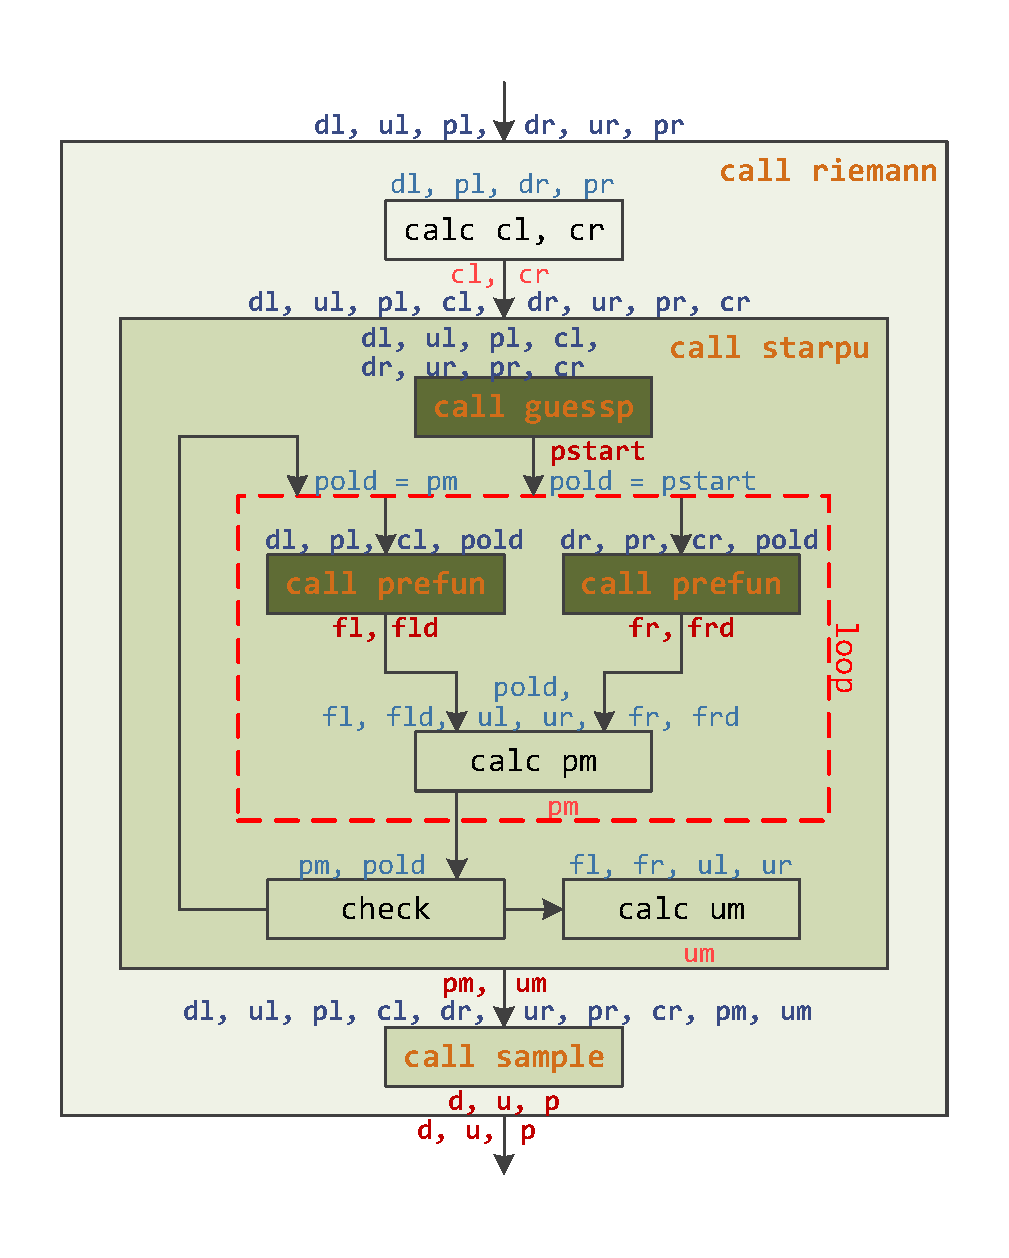
\includegraphics[width=8cm]{pics/pic_functions}
\caption{Data flow diagram in Riemann solver}
\label{pic:functions}
\end{figure}

Fig.~\ref{pic:functions} shows a diagram of the work of the Riemann solver with the indicated data streams and calls of all the functions involved in the implementation. The \texttt{riemann} function calculates the speed of sound on the right and left, performs a vacuum test, and subsequently calls the \texttt{starpu} and \texttt{sample} functions.
The \texttt{starpu} function calculates the velocity and pressure values in the middle region between the left and right waves (star region), and the function contains a cycle with an unknown number of iterations to solve a non-linear equation by the iterative Newton method, inside which there are calls to other functions (\texttt{prefun}).
The \texttt{guessp} and \texttt{prefun} functions contain only arithmetic calculations and simple conditions and are the simplest from the point of view of vectorization.
Finally, the last \texttt{sample} function determines the final gap configuration by calculating a set of conditions.
This function contains a very branched control, the nesting of conditions in it reaches four, which makes it difficult to use vectorization.

In the counting process, a number of calls to the \texttt{riemann} function with different sets of input data are made using numerical methods based on the Riemann solver (during each counting iteration, one call is made for each face of each cell of the computational grid).
Since the riemann function is pure, calls for different input data sets (\texttt{dl}, \texttt{ul}, \texttt{pl}, \texttt{dr}, \texttt{ur}, \texttt{pr}) are independent and there is a desire to merge calls for the purpose of effective use of vector (element-wise) instructions.
As such a combined call, we will consider a function in which, instead of atomic data of the type \texttt{float}, the corresponding vectors containing 16 elements each are passed.

\begin{equation}\label{eq:riemann_16}
\overline{U_l} = \left( \begin{array}{ccc} \overline{d_l} \\ \overline{u_l} \\ \overline{p_l} \end{array} \right),
\overline{U_r} = \left( \begin{array}{ccc} \overline{d_r} \\ \overline{u_r} \\ \overline{p_r} \end{array} \right),
\overline{U} = \left( \begin{array}{ccc} \overline{d} \\ \overline{u} \\ \overline{p} \end{array} \right) = riem(\overline{U_l}, \overline{U_r})
\end{equation}

In the formula (\ref{eq:riemann_16}), all variables $\overline{d_l}$, $\overline{u_l}$, $\overline{p_l}$, $\overline{d_r}$, $\overline{u_r}$, $\overline{p_r}$, $\overline{d}$, $\overline{u}$, $\overline{p}$ are vectors of length 16.
For example, the vector $\overline{d}$ contains 16 values of gas density, obtained by solving 16 Riemann problems combined into one challenge.
This also applies to other variables.

At the same time, it is possible to perform the same actions with vector data as with basic types - perform calculations, pass to functions, and return as a result.
In the process of optimization, for clarity, we will avoid substitution of the function body into the call point.
Thus, as a result of vectorization, our goal is to obtain vector analogs of all the functions used in the Riemann solver which were described above.

\section{Simple context vectorization}

The simplest context for computing vectorization when combining calls is the \texttt{prefun} function (the \texttt{guessp} function has similar properties and is not considered).
A non-vectorized version of the function is presented in Fig.~\ref{pic:prefun_code}.

\begin{figure}
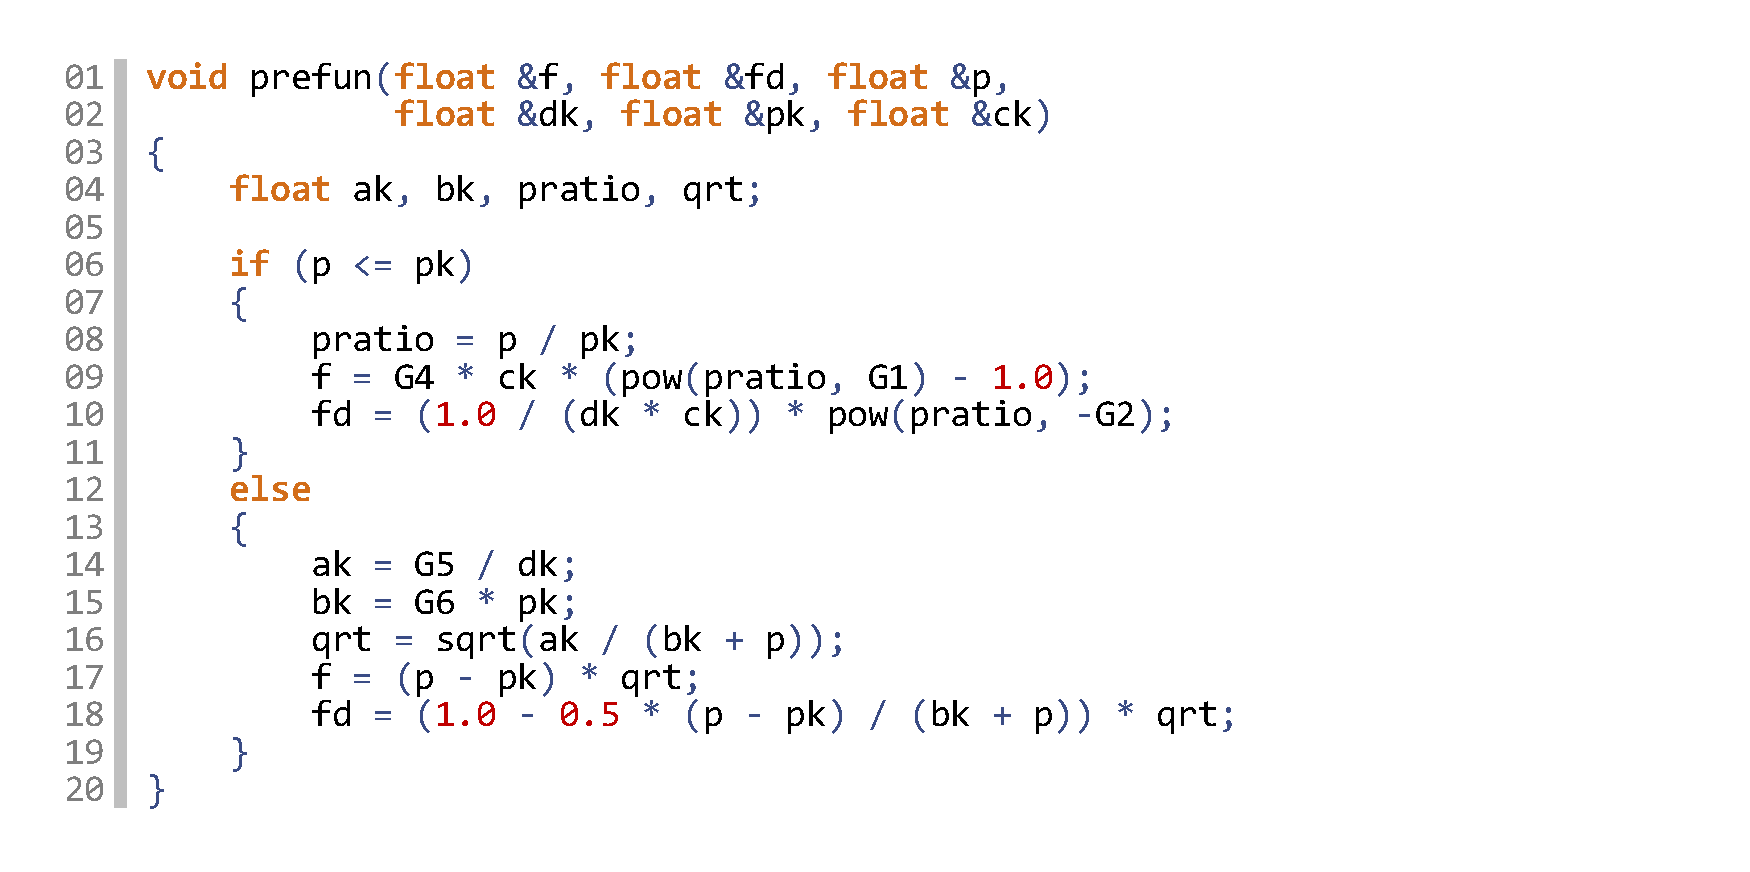
\includegraphics[width=10cm]{pics/pic_prefun_code}
\caption{Original version of the function \texttt{prefun}}
\label{pic:prefun_code}
\end{figure}

This code contains only simple arithmetic operations, square root extraction, exponentiation and comparison.
For all these actions, vector equivalents are provided in the AVX-512 command set.
The function code is vectorized by replacing arithmetic operations with vector analogs.
The calculation of values under the condition (\texttt{if-else}) is vectorized by using vector predicates obtained using vector comparison (see Fig.~\ref{pic:prefun_16_code}).
Three points are worth noting in the vectorization of the \texttt{prefun} function.

\begin{figure}
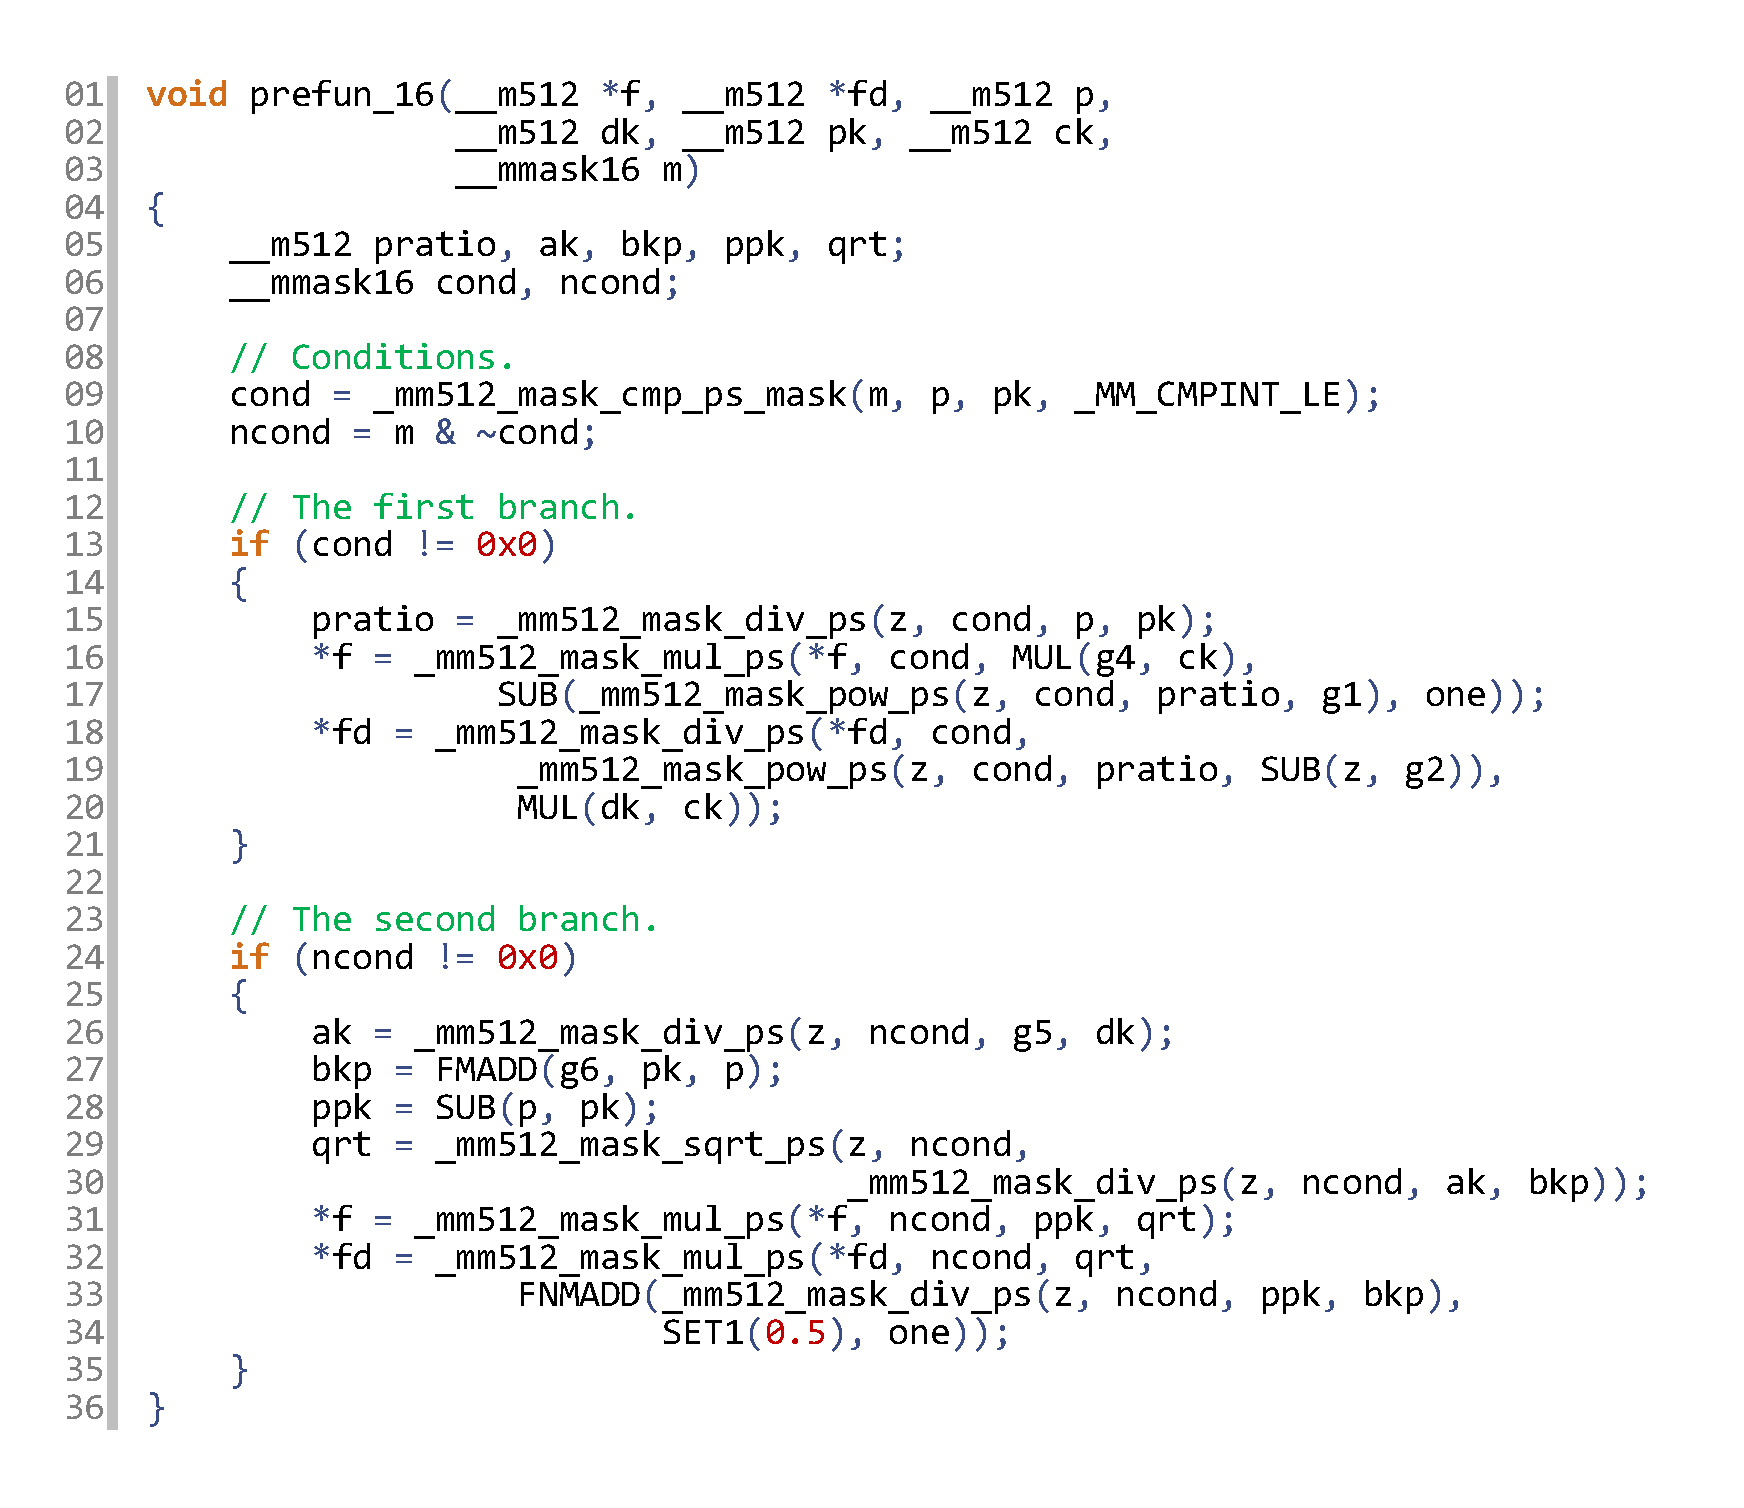
\includegraphics[width=10cm]{pics/pic_prefun_16_code}
\caption{Vectorized version of the function \texttt{prefun}}
\label{pic:prefun_16_code}
\end{figure}

Since the vector division operation is slow, the following identities were used to reduce the number of divisions:

\begin{equation}\label{eq:deldel}
\frac{a}{\frac{b}{c}} = \frac{ac}{b}, \frac{\frac{a}{b}}{c} = \frac{a}{bc}
\end{equation} 

Since the \texttt{prefun} function is called inside the loop in the \texttt{starpu} function, an additional mask argument must be added to its implementation, by which the elements processed in this call are selected (Fig.~\ref{pic:prefun_16_code} line 03).
This will be described in more detail below, when the vectorization of the \texttt{starpu} function will be discussed.

One more important point of vectorization is optimization of work with conditions.
In the process of performing vectorization, we have formed two groups of vector instructions executed under the predicates \texttt{cond} (Fig.~\ref{pic:prefun_16_code}, lines 15-20) and \texttt{ncond} (Fig.~\ref{pic:prefun_16_code}, lines 26-34).
Since physical tasks are characterized by continuous changes in physical quantities, it can be argued that the data sets processed in a vectorized call are similar.
In other words, all the vectors involved in the calculations contain similar values.
The same statement applies to predicate vectors.
Indeed, the execution statistics shows that for physical tasks the most frequent values of the predicate vectors (in this case, \texttt{cond} an \texttt{ncond}) are the values \texttt{0x0} and \texttt{0xFFFF}.
Thus, checks of predicate vector registers for emptiness (Fig.~\ref{pic:prefun_16_code}, lines 13 and 24) immediately cut off entire blocks of unnecessary operations performed with a zero mask.

\section{Vectorization of highly branched conditions}

\begin{figure}
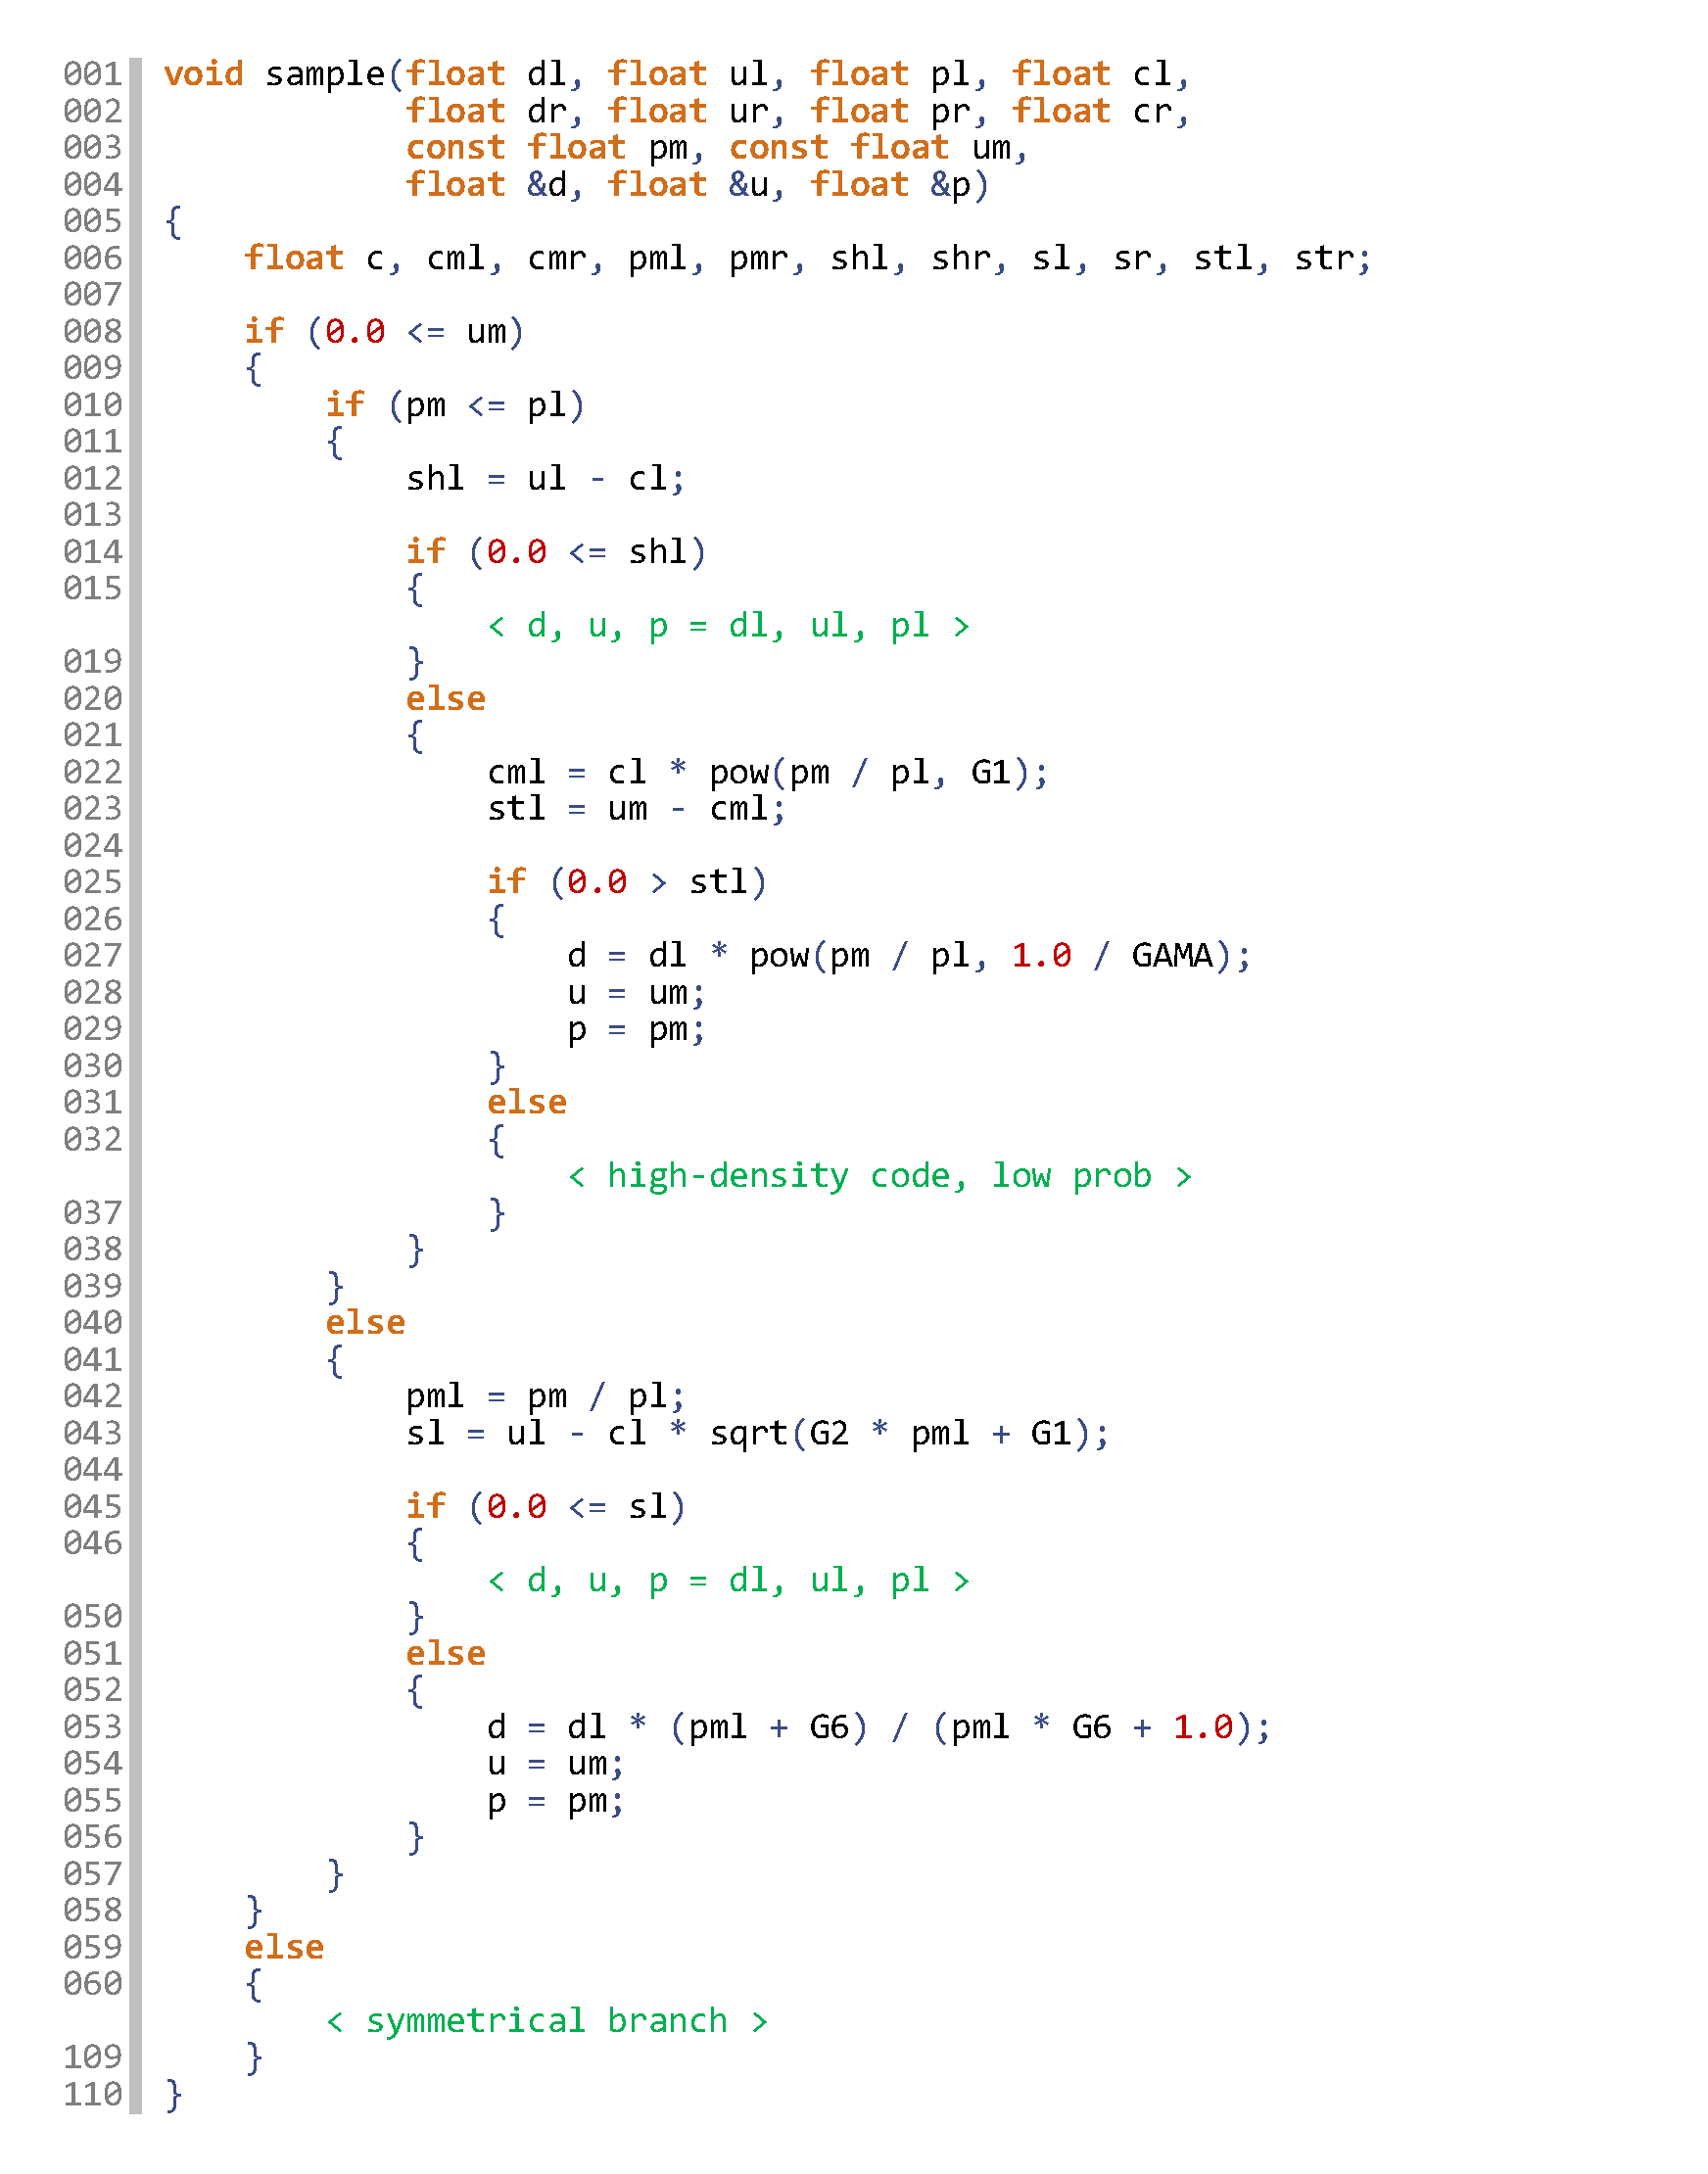
\includegraphics[width=10cm]{pics/pic_sample_code_4}
\caption{Original version of the function \texttt{sample}}
\label{pic:sample_code_4}
\end{figure}

The \texttt{sample} function contains a highly branched control with a nesting level of 4 (see Fig.~\ref{pic:sample_code_4}).
The condition tree built for this function contains 10 leaf nodes, in each the value of the gas-dynamic values \texttt{d}, \texttt{u}, \texttt{p} is determined.
Direct computation of the vector predicates of all leaf nodes and the execution of their code under these predicates slows down the resulting code, so the following actions were performed when vectoring this function.

First, it was noted that the 4 linear sections contain the definition of the gas-dynamic parameters \texttt{d}, \texttt{u} and \texttt{p}, which could be changed to initialization by removing the assignment operations upward through the function code.
Thus, 4 linear sections were deleted.
This initialization of the parameters \texttt{d}, \texttt{u}, \texttt{p} does not contain arithmetic operations (the parameters are initialized by the arguments of the function \texttt{dl}, \texttt{ul}, \texttt{pl} or \texttt{dr}, \texttt{ur}, \texttt{pr}), which means it can be performed using vector merge operations \texttt{blend}.

It was further noted that the \texttt{sample} function handles the right and left profiles of the breakup decay in the same way with minor changes.
Using a simple replacement of variables, which consists in changing the sign of the velocity value, we managed to merge the code for two subtrees, based on the condition \texttt{pm} $\le$ \texttt{pl}, which reduced the amount of the calculation code by half and expectedly reduced the time execution by 45\%.

\begin{figure}
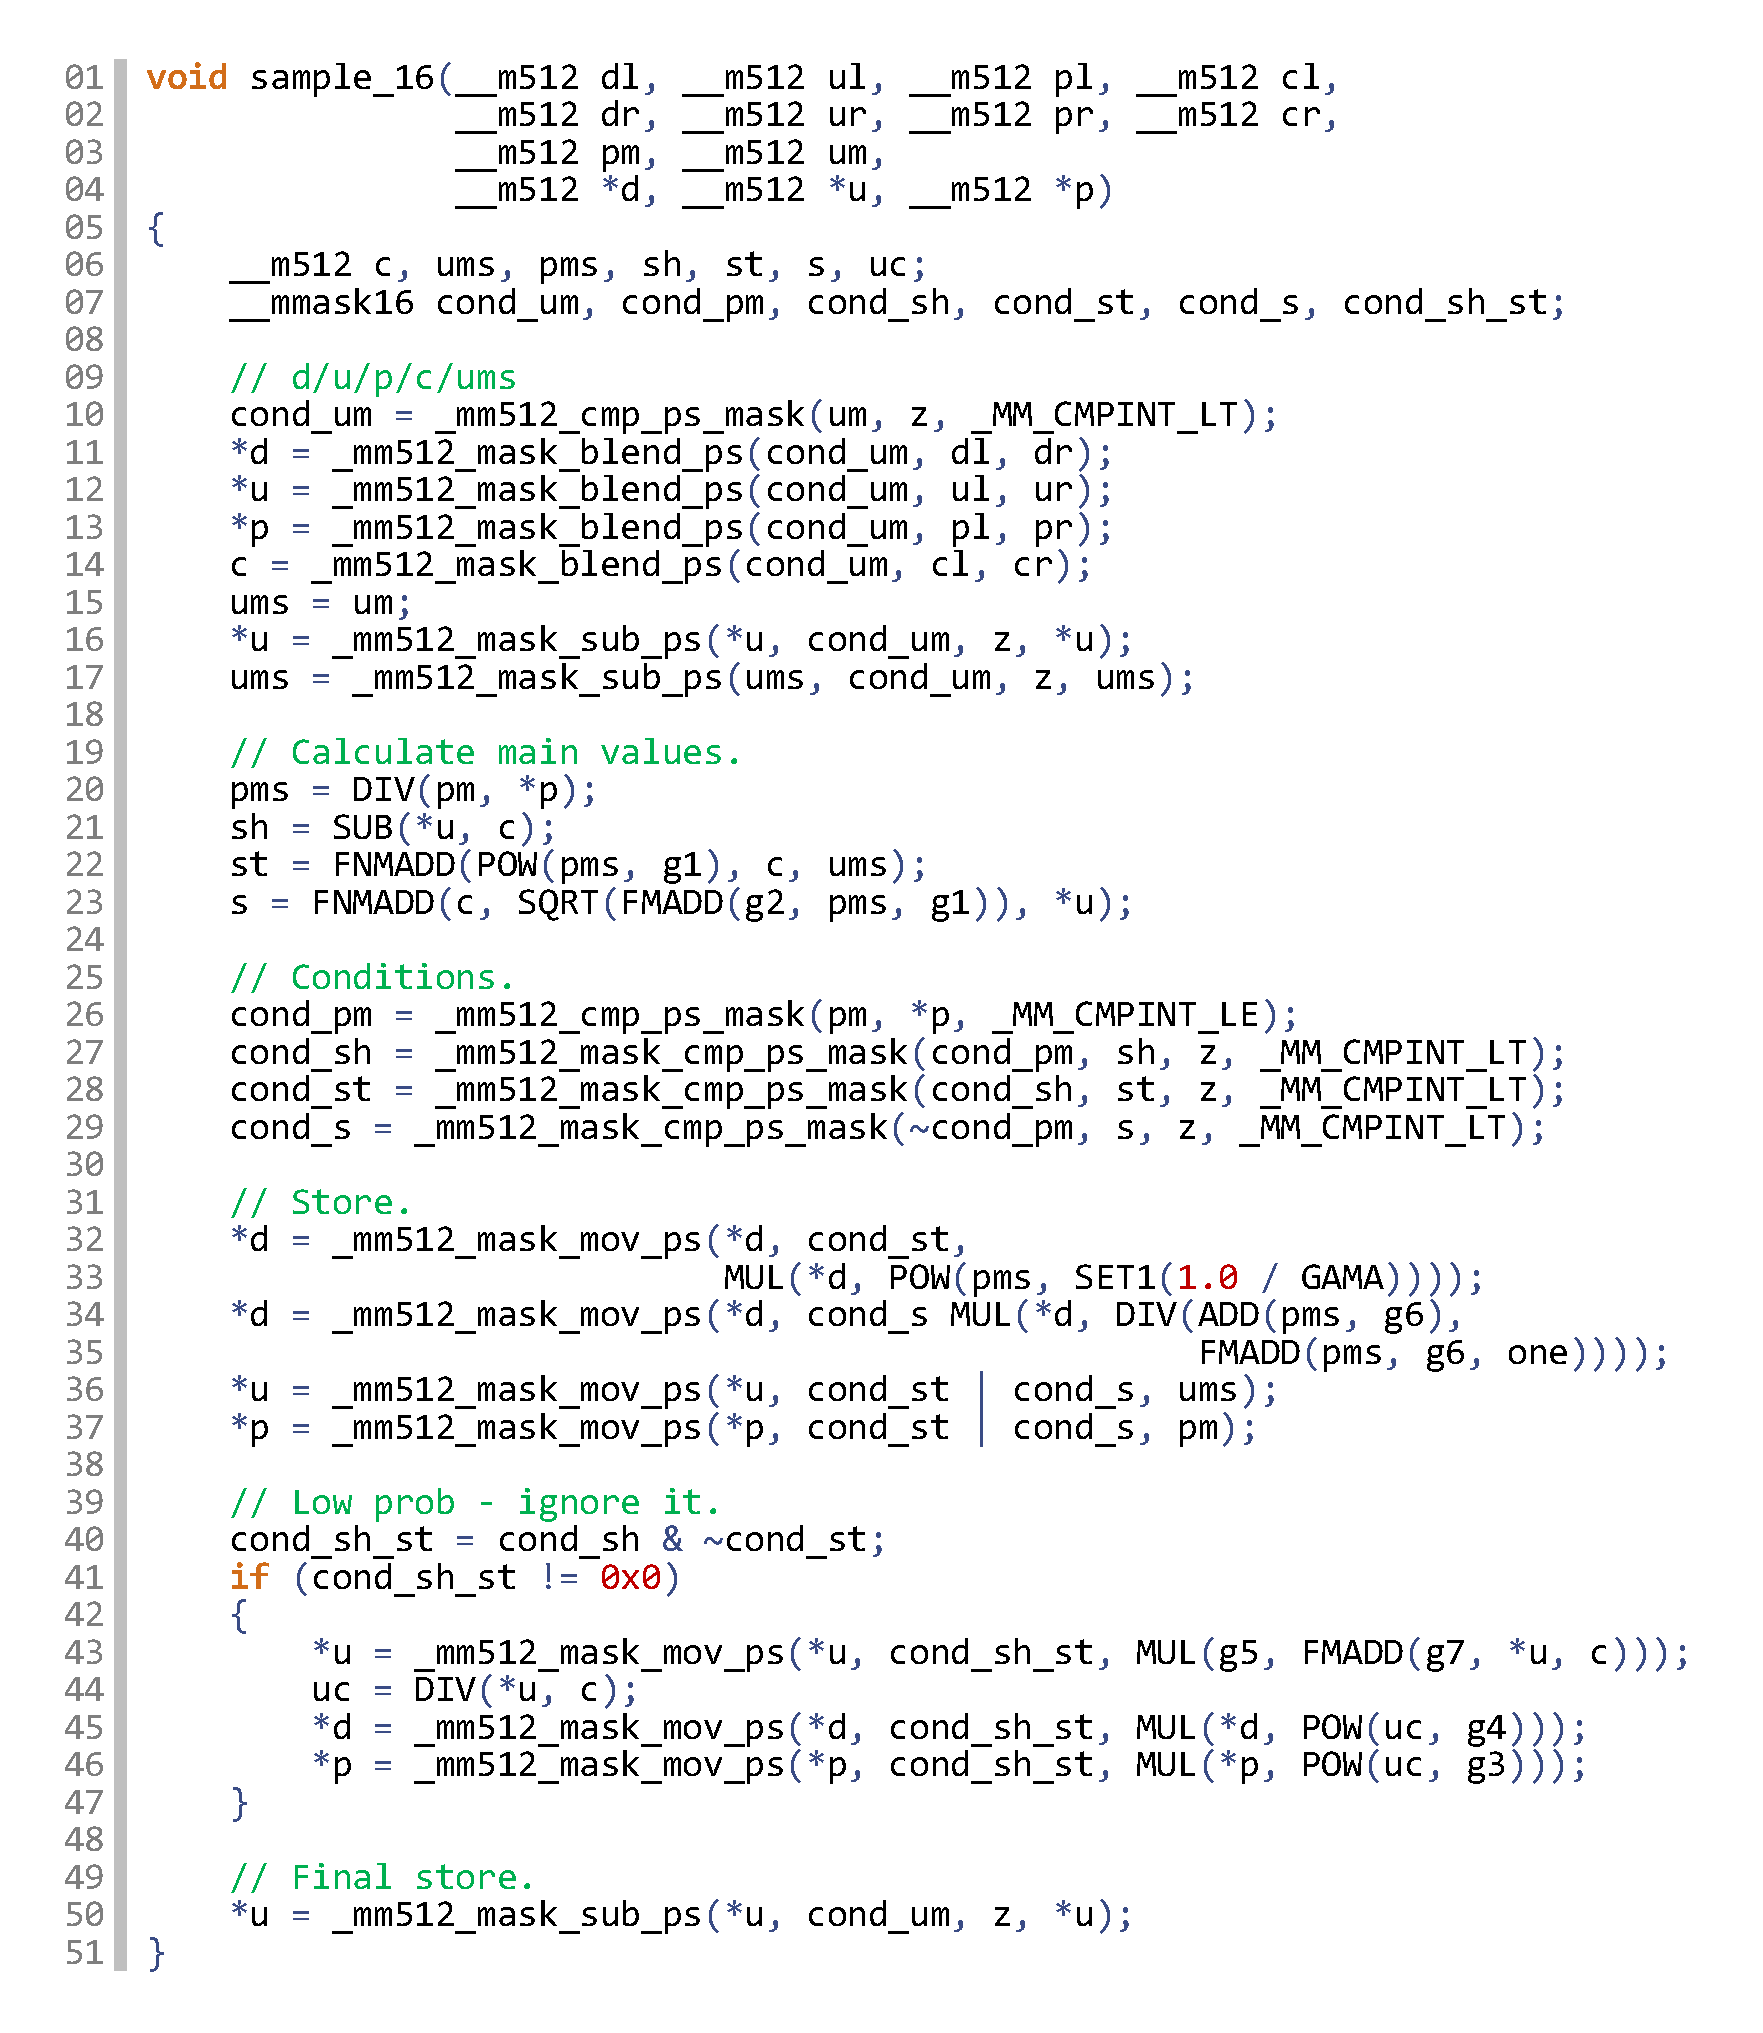
\includegraphics[width=10cm]{pics/pic_sample_16_code}
\caption{Vectorized version of the function \texttt{sample}}
\label{pic:sample_16_code}
\end{figure}

After the reduction of the code, the number of leaf nodes in the conditions tree was reduced to three.
However, even in this case, direct merging of the code using vector predicates turned out to be ineffective.
This was caused by the unlikely part of the code, heavy operations, among which there are calls to the function of raising to a power (Fig.~\ref{pic:sample_code_4}, lines 033-036).
The vector predicate of this code segment in more than 95 percent of cases has the value \texttt{0x0}, therefore, before executing this code segment, it is advisable to check this predicate for emptiness (which corresponds to the removal of the unlikely branch of execution from the function body).
The removal of an unlikely branch of execution from the main program context can significantly speed up the executable code, since the presence of a large number of such rare computations can serve as a reason for refusing vectorization \cite{RybLowProb}.

For the rest of the code, the merge can be done with the remarks described in the previous section.
As a result, the vectorized sample function was accelerated more than 10 times.
The final vector code is presented in Fig.~\ref{pic:sample_16_code}.
In this code, lines 11–14 correspond to initialization, lines 16, 17, and 50 are responsible for replacing the variables for merging symmetric sections of the code, and the unlikely branch is separated in the block located in lines 41–47.

\section{Loop nests vectorization}

\begin{figure}
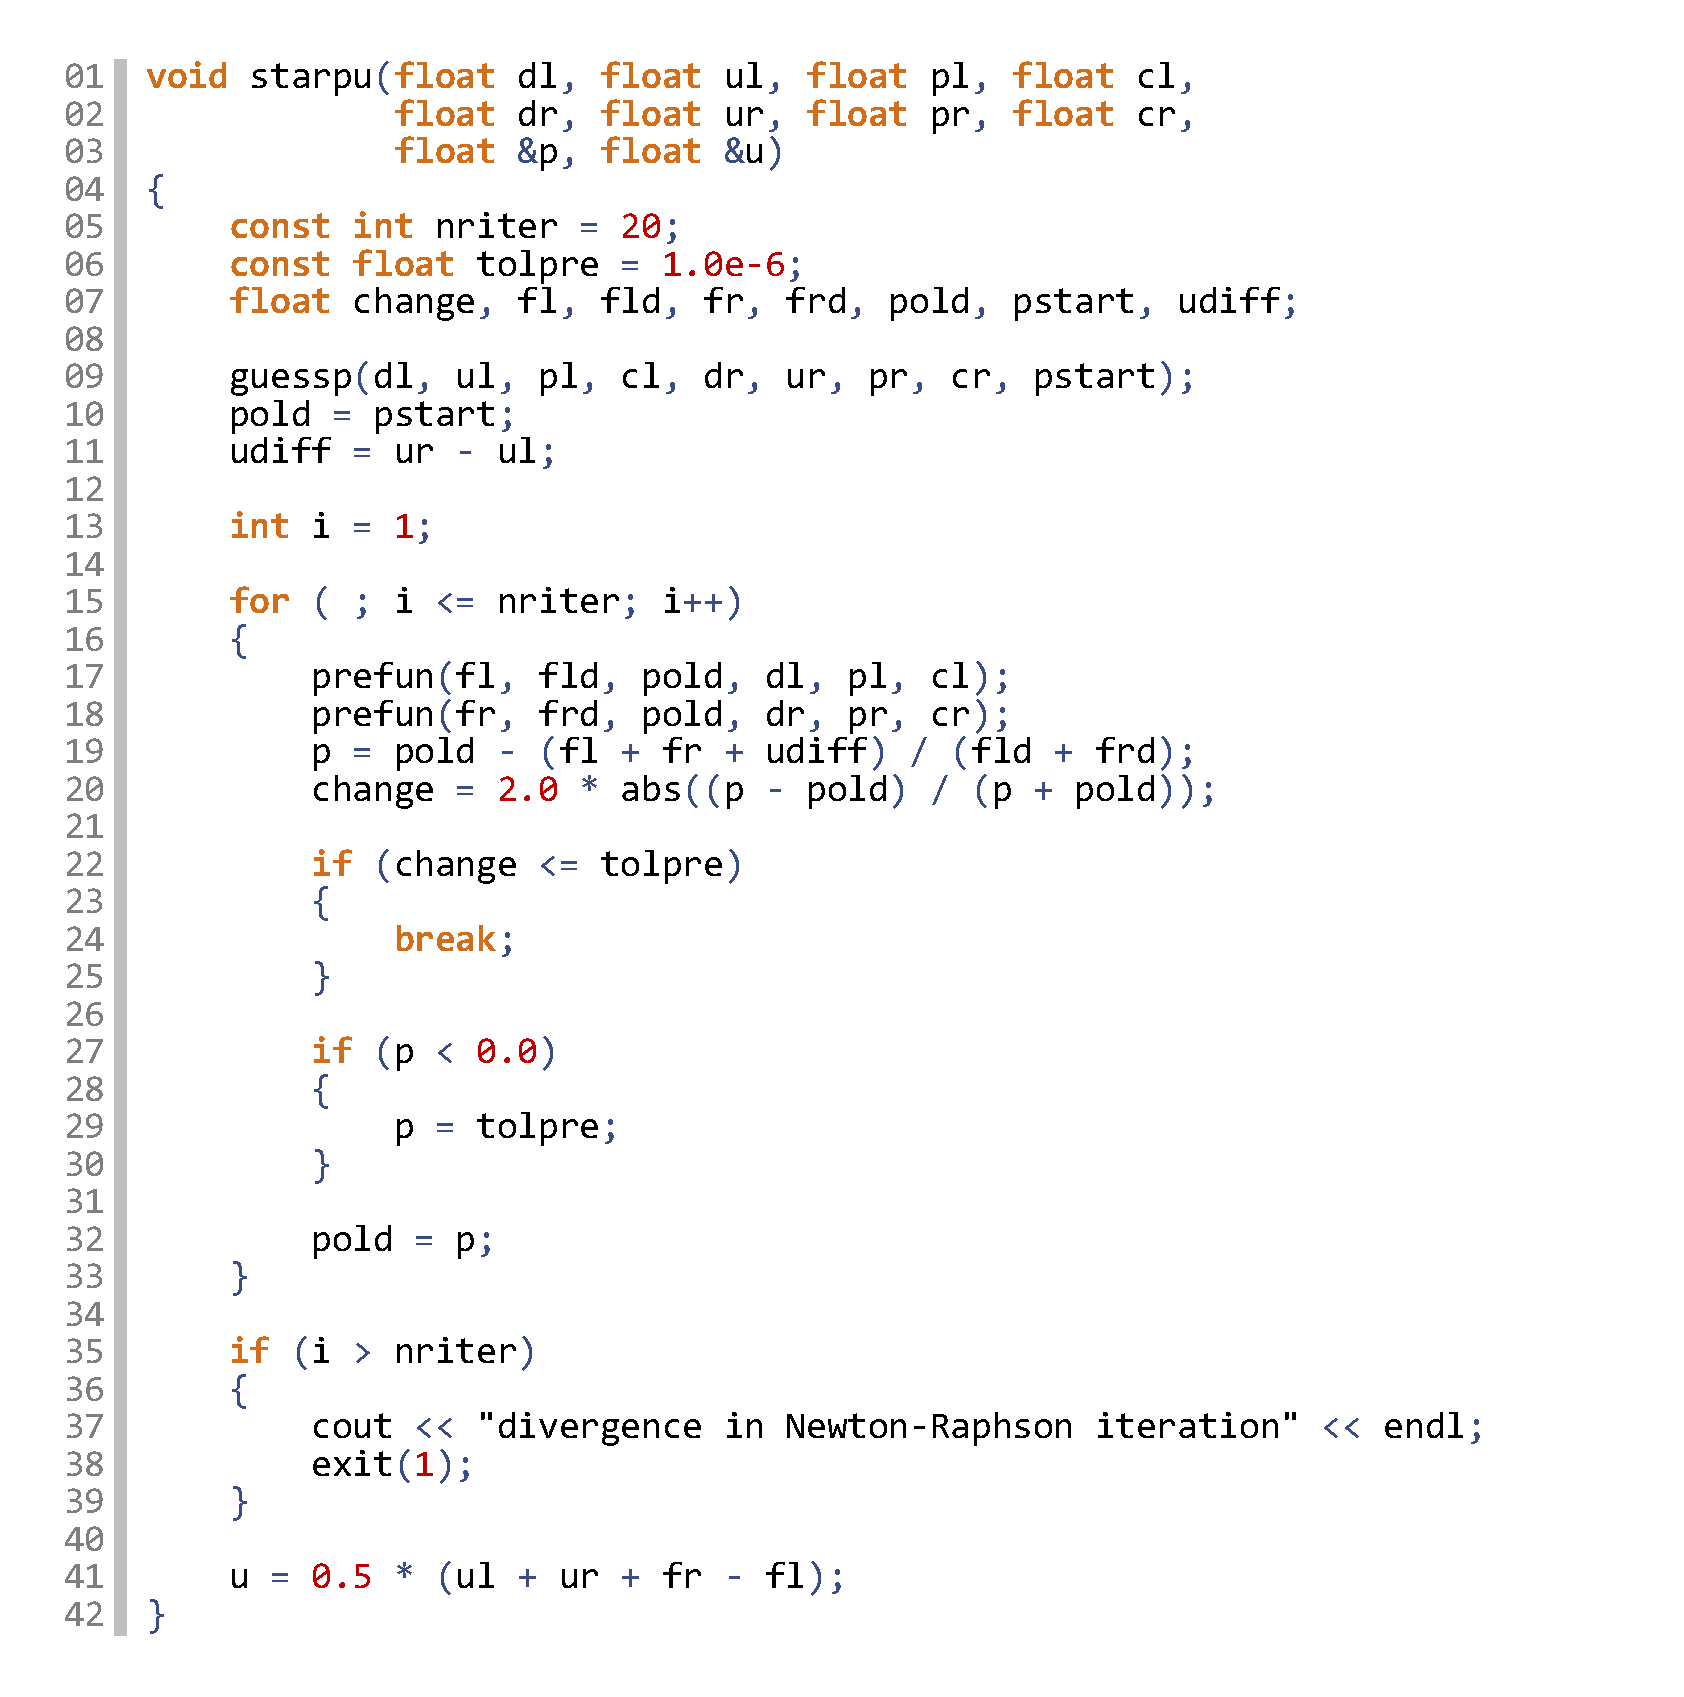
\includegraphics[width=10cm]{pics/pic_starpu_code}
\caption{Original version of the function \texttt{starpu}}
\label{pic:starpu_code}
\end{figure}

The most complex context for code vectorization is the \texttt{starpu} function, which contains a loop with an unknown number of iterations (Fig.~\ref{pic:starpu_code}).
The loop located in this function in lines 15-33, in addition to an unknown number of iterations, also contains conditional transitions (\texttt{if, break}) and calls of \texttt{prefun} functions, which also complicates its vectorization.
Before performing vectorization, this cycle must be transformed into a predicate form, in which the body should not contain transition operations.
All cycle instructions are executed under their predicates, and the execution of the cycle is interrupted if all predicates are zeroed.
This mechanism is described in \cite{RybTelShabLoopsVect} in relation to the vectoring of Shell sort and in \cite{Krzikalla} in relation to the Mandelbrot set construction.
At the same time, it is worth noting that calls to prefun functions must also have corresponding predicates.
After the body of the cycle is transformed into a predicate form, it can be vectorized, after which the predicates of the instructions are replaced by vector mask registers (this is where the additional parameter of the vectorized function \texttt{prefun} appears in the form of a mask).
The result of the \texttt{starpu} function vectorization is presented in Fig.~\ref{pic:starpu_16_code}.
Line 18 shows the initial initialization of the full mask for performing vectorized loop iterations. As the cycle works, the mask is exhausted (line 32), and when it is fully zeroed, the cycle ends.

\begin{figure}
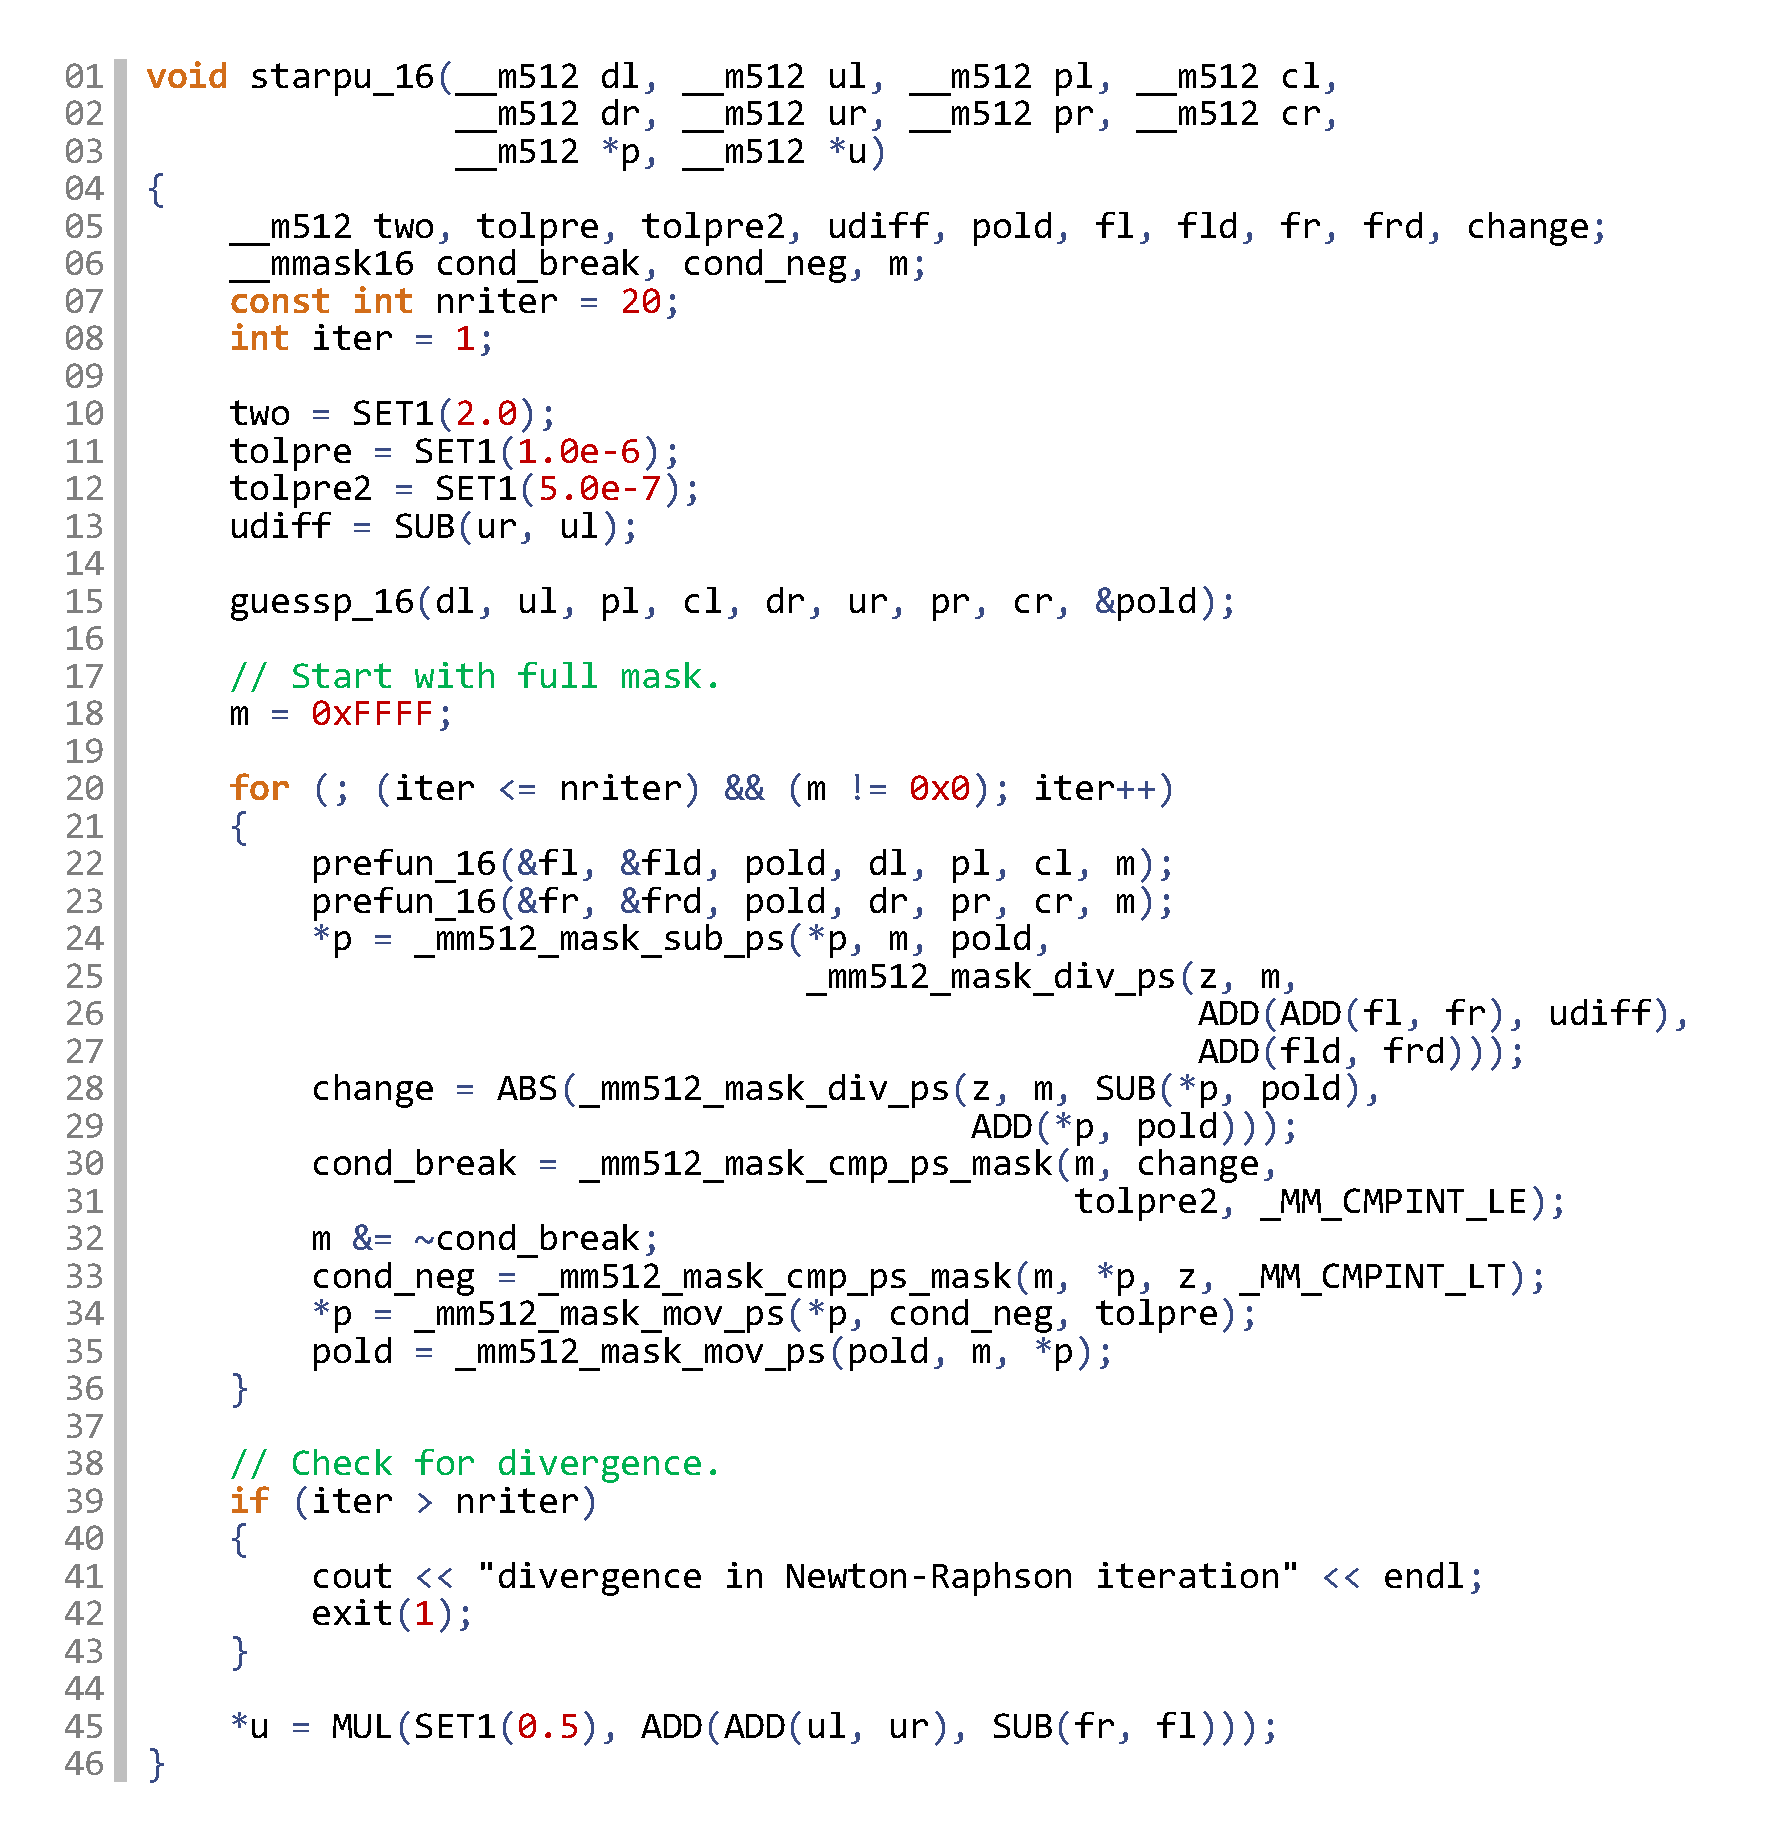
\includegraphics[width=10cm]{pics/pic_starpu_16_code}
\caption{Vectorized version of the function \texttt{starpu}}
\label{pic:starpu_16_code}
\end{figure}

It should be noted that the vectorization of a loop with an unknown number of iterations can be quite dangerous, since the number of iterations of a vectorized cycle is equal to the maximum of the iterations number of the cycles with 16 combined calls of the original non-vectorized function.
If there is a big difference in the number of iterations of the original code, there is a drop in efficiency due to the low density of the masks of the executable instructions, as shown in \cite{RybTelShabLoopsVect}.

\section{Results analysis}

Before starting the optimization of the program code of the Riemann solver, an execution profile was collected, which showed that the execution time was distributed between individual functions according to the diagram presented in Fig.~\ref{pic:exe_prof}.

\begin{figure}
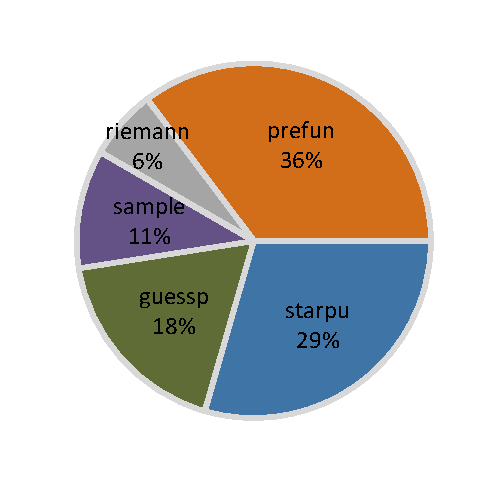
\includegraphics[width=8cm]{pics/pic_exe_prof}
\caption{The distribution of the execution time of the Riemann solver between individual functions}
\label{pic:exe_prof}
\end{figure}

To collect the execution profile, the source program was compiled with the prohibition of optimizing the substitution of the function body into the call point (inline).
Thus, the diagram shows the net execution time of functions without taking into account nested calls.
It can be seen from the diagram that the largest share of the execution time falls on the \texttt{prefun} function (36\%), which contains a simple program context with one condition.
Also, a significant part of the execution time falls on the \texttt{starpu} function (29\%), which contains a loop nest with an unknown number of iterations.
The remaining time is divided between the three other functions \texttt{guessp} (18\%), \texttt{sample} (11\%), \texttt{riemann} (6\%).

The approaches to the vectorization of the Riemann solver functions described in the article were implemented in the C programming language using the intrinsics functions and tested on the Intel Xeon Phi 7290 microprocessors that are part of the computing segment knl of the MVS-10P supercomputer located in JSCC RAS.

Performance testing was carried out on the input data arrays collected in solving standard test problems: the Soda problem, the Lax problem, the weak shock wave problem, the Einfeldt problem, the Woodward-Colella problem, the Schu-Osher problem and others \cite{BulVolTest}.

The diagram Fig.~\ref{pic:perf} shows the effect of applying various optimizations to each of the functions in question, as well as the total acceleration obtained as a result of vectorization.

\begin{figure}
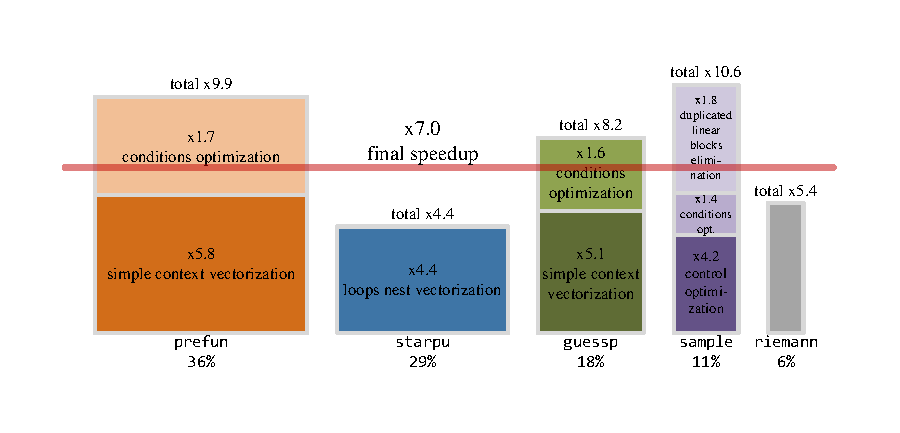
\includegraphics[width=12cm]{pics/pic_perf_eng}
\caption{The acceleration diagram of individual functions and the total acceleration of the Riemann solver}
\label{pic:perf}
\end{figure}

It can be noted that the effect of the vectorization of a simple context varies from 5.1 to 5.8 times (for the functions \texttt{guessp} and \texttt{prefun}).
It should also be noted a significant effect of the optimization of conditions (check on the emptiness of the mask of predicates, under which the execution of the block of operations is located).
This is a fairly simple conversion, which accelerates the code from 1.4 to 1.7 times (for the functions \texttt{sample} and \texttt{prefun}) depending on how close the conditions are from adjacent iterations of the vectorized loop.

Separately, the diagram emphasizes the effect of applying variable optimization, which allowed the \texttt{sample} function to be accelerated 1.8 times by merging two subtrees of the control flow graph (that is, duplicate linear sections were removed).

As a result of applying all the described optimizations, it was possible to achieve acceleration of individual sections of the program execution 10 or more times, and the total acceleration of the entire Riemann solver was 7 times (marked with a red line in Figure~\ref{pic:perf}).

\section{Related works}

Here is a brief comparison of the results obtained in this article with the results of other works aimed at improving the efficiency of the Riemann solvers on parallel architectures.
At the same time, we note that although the work did not consider the parallelization of numerical methods based on the Riemann solver using MPI, OpenMP, as well as using graphics accelerators, it would be wrong not to mention the works concerning these aspects of parallelization.

The work \cite{Shumlak} considers an algorithm for numerically solving the equations of magnetohydrodynamics based on the approximate Riemann solver, developed by Roe.
In this case, the calculations are carried out on a block-structured computational grid, and for parallelization using MPI, the blocks of the grid are decomposed (cutting along one or several directions).
The results of measuring the indicator of weak scalability when using up to 16 processors are presented.
This indicator is close to unity and even in some cases exceeds it.
Such a phenomenon, called superlinear scalability, can also be found in other works devoted to the parallelization of numerical methods of gas dynamics, for example, in \cite{Benderskij}.

The work \cite{Schive} is devoted to parallelizing numerical methods based on various approximate Riemann solvers for execution on NVIDIA Tesla C2050 graphics accelerators.
In addition to the Roe solver, the HLLE and HLLC \cite{Kong} solvers are also used.
Methods are demonstrated that allow achieving acceleration on a graphics accelerator compared to the Intel Xeon E5530 processor by 101 times using a uniform grid.
The indicators of weak and strong scalability of a parallelized application using 32 GPUs are also given, they amounted to 98.8\% and 85.0\%, respectively.

The work \cite{Mandli} presents the results of using the PetClaw tool (a Python shell integrating the Clawpack computing core written in Fortran and the PETSc library into a single parallel application) for parallelizing hydrodynamic calculations using MPI to a large number of cores, up to 16 thousand.
At the same time, a parallelization efficiency indicator close to unity was demonstrated.

The works \cite{Kulikov}, \cite{Kulikov2} describe approaches to parallelizing computations for modeling astrophysical flows on hybrid supercomputers equipped with Intel Xeon Phi accelerators.
In particular, 134-fold acceleration of computational codes on one accelerator was demonstrated using multi-threaded parallelization, as well as 75\% scalability when using up to 224 accelerators.
The article notes that to further accelerate the application, a vectorization of the computing core is needed and a forecast is given to achieve 80\% peak performance provided that vectorization is applied.

Closest to this work are \cite{BaderSWEVect}, \cite{FerreiraSWEVect}, in which special attention is paid to the vectorization of the Riemann solver for the numerical solution of shallow water equations.
The work \cite{BaderSWEVect} presents results on acceleration of 6-7 times when vectorizing a Riemann solver for a given single precision on Intel Xeon Phi KNC accelerators.
In \cite{FerreiraSWEVect}, the vectorization method was improved and the effect was already 2.4-6.5 in double-precision operations on Intel Xeon Phi KNL microprocessors.
However, these works use a specially developed approximate Riemann solver for shallow water equations \cite{George}.
The implementation of this solver contains a simpler computational context compared to the exact solver, whose vectorization is considered in the current work.
The approximate solver from \cite{George} contains only arithmetic operations and can be automatically vectorized after special preparation of input parameters (grouping several solver calls into one call with vector parameters).

Based on a comparison of current work with related work in this area, it can be noted that the acceleration rate of the exact Riemann solver, equal to 7 and achieved by vectorizing the program code using the AVX-512 instruction set, can be considered acceptable.

\section*{Conclusion}

The paper examined approaches to vectorizing complex program contexts using the AVX-512 instruction set.
This instruction set appeared in Intel microprocessors starting with Intel Xeon Phi KNC accelerators, and then entered Intel Xeon Phi KNL microprocessors, Intel Xeon Phi Skylake and beyond.
The AVX-512 instructions support predicate processing of data elements, which allows you vectorize complex, branched program code with them.

The exact Riemann solver was used as the target task, since it has a compact implementation but at the same time contains features that prevent automatic vectorization by means of the compiler (function calls, complex control, nested loops).
For vectorization, an approach was used in which several consecutive calls to the solver function were replaced with one call with vector parameters (and with corresponding changes to the function body).
This allowed several instances of the task to be performed simultaneously on the same processor core (the number of instances equals the width of the vector, in this case 16).

The components of the Riemann solver were analyzed, their features were highlighted, and a method of effective vectorization was proposed for each of them.
As a result of vectorization, acceleration was achieved more than 10 times in individual sections of the solver, and the final acceleration was 7 times on the data with single precision.

The developed methods of vectorization of a complex program context can be used to optimize other computational problems.
In particular, at present, a team of authors of this article is developing a library aimed at vectorization of arbitrary flat cycles, that is, cycles in which there are no inter-iteration dependencies.
In this case, the body of the loop can include elements such as complex control, loop sockets, calls to pure functions, goto statements, and others.
The implementation of such a tool will significantly improve the performance of calculation codes, the automatic vectorization of which by the compiler is impossible.

The work was done at the JSCC RAS as part of the state assignment on the topic 0065-2019-0016 (registration number AAAA-A19-119011590098-8). 

\begin{thebibliography}{30}

\bibitem{KulPogSemRiemann}
\by A. G. Kulikovskiy , N. V. Pogorelov, A. Y. Semenov
\book Matematicheskiye voprosy chislennogo resheniya giperbolicheskikh sistem uravneniy [Mathematical Aspects of Numerical Solution of Hyperbolic Systems]
\yr 2001
\publ FIZMATLIT
\publaddr Moscow
\totalpages 608

\bibitem{BorRykRiemann}
\by V. E. Borisov, U. G. Rykov
\preprint Tochnyy rimanovskiy solver v algoritmakh resheniya zadach mnogokomponentnoy gazovoy dinamiki
\preprintinfo Preprints of the IAM named after M. V. Keldysh 96
\yr 2018 
\totalpages 28
\URL http://library.keldysh.ru/preprint.asp?id=2018-96
\crossref{http://dx.doi.org/10.20948/prepr-2018-96}

\bibitem{Godunov}
\by S. K. Godunov, A. V. Zabrodin, M. Y. Ivanov, A. N. Krayko, G. P. Prokopov
\book Chislennoye resheniye mnogomernykh zadach gazovoy dinamiki [Numerical solution of multidimensional problems of gas dynamics]
\yr 1976
\publ Nauka
\publaddr Moscow
\totalpages 400

\bibitem{Shumlak}
\by U. Shumlak, B. Udrea
\paper An approximate Riemann solver for MHD computations on parallel architectures
\jour Proceedings of the 15th AIAA Computational Fluid Dynamics Conference
\yr 2001
\crossref{http://dx.doi.org/10.2514/6.2001-2591}

\bibitem{Schive}
\by H. Y. Schive, U. H. Zhang, T. Chiueh
\paper Directionally unsplit hydrodynamic schemes with hybrid MPI/OpenMP/GPU parallelization in AMR
\jour International Journal of High Performance Computing Applications
\yr 2011
\pages 367-377
\crossref{http://dx.doi.org/10.1177/1094342011428146}

\bibitem{Mandli}
\by K. T. Mandly, A. Alghamdi, A. Ahmadia, D. I. Ketcheson, W. Scullin
\paper Using Python to construct a scalable parallel nonlinear wave solver
\jour Proceedings of the 10th Python in Science Conference (SCIPY 2011)
\yr 2011
\pages 61-66

\bibitem{Kulikov}
\by I.M. Kulikov, I.G. Chernykh, E.I. Vorobyev, A.V. Snytnikov, D.V.Vins and others
\paper Chislennoye gidrodinamicheskoye modelirovaniye astrofizicheskikh techeniy na gibridnykh SuperEVM, osnashchennykh uskoritelyami Intel Xeon Phi
\jour Superkomp'yuternoye modelirovaniye 
\yr 2016
\vol 5
\issue 4
\pages 77-97
\crossref{http://dx.doi.org/10.14529/cmse160406}

\bibitem{Kulikov2}
\by I. Kulikov, I. Chernykh, V. Vshivkov, V. Prigarin, V. Mironov, A. Tatukov
\paper The parallel hydrodynamic code for astrophysical flow with stellar equation of state
\jour Proceedings of Russian Supercomputing Days 2018
\pages 612-624

\bibitem{BaderSWEVect}
\by M. Bader, A. Breuer, W. H{\"o}ltz, S. Rettenberger
\paper Vectorization of an augmented Riemann solver for the shallow water equations
\jour Proceedings of the 2014 International Conference on High Performance Computing and Simulation, HPCS 2014
\yr 2014
\pages 193-201
\crossref{http://dx.doi.org/10.1109/HPCSim.2014.6903686}

\bibitem{FerreiraSWEVect}
\by C. R. Ferreira, K. T. Mandli, M. Bader
\paper Vectorization of Riemann solvers for the single- ans multi-layer shallow water equations
\jour Proceedings of the 2018 International Conference on High Performance Computing and Simulation, HPCS 2018
\yr 2018
\pages 415-422
\crossref{http://dx.doi.org/10.1109/hpcs.2018.00073}

\bibitem{VolOkuPred}
\by V. Y. Volkonskiy, S. K. Okunev
\paper Predikatnoye predstavleniye kak osnova optimizatsii programmy dlya arkhitektur s yavno vyrazhennoy parallel'nost'yu
\jour Informatsionnyye tekhnologii
\yr 2003
\issue 4
\pages 36-45

\bibitem{KimElbrus}
\by A. K. Kim, V. I. Perekatov, S. G. Yermakov
\book Mikroprotsessory i vychislitel'nyye kompleksy semeystva <<Elbrus>>[Microprocessors and computing complexes of the << Elbrus >> family]
\yr 2013
\publ Piter
\publaddr Saint Petersburg
\totalpages 273

\bibitem{IntelIntrGuide}
\finalinfo Intel Intrinsics Guide\\
\href{https://software.intel.com/sites/landingpage/IntrinsicsGuide/}{{\tt https://software.intel.com/sites/landingpage/IntrinsicsGuide/}}

\bibitem{TorRiemann}
\by E. F. Toro
\book Riemann Solvers and Numerical Methods for Fluid Dynamics: A Practical Introduction
\edition 2 nd Edition
\yr 1999
\publ Springer
\totalpages 645

\bibitem{Numerica}
\finalinfo NUMERICA, A Library of Sources for Teaching, Research and Applications, by E. F. Toro
\href{https://github.com/dasikasunder/NUMERICA}{{\tt https://github.com/dasikasunder/NUMERICA}}

\bibitem{RybLowProb}
\by A. A. Rybakov
\paper Optimizatsiya zadachi ob opredelenii konfliktov s opasnymi zonami dvizheniya letatel'nykh apparatov dlya vypolneniya na Intel Xeon Phi
\jour Programmnyye produkty i sistemy
\yr 2017
\vol 30
\issue 3
\pages 524-528
\URL http://www.swsys.ru/index.php?page=article&id=4325
\crossref{http://dx.doi.org/10.15827/0236-235.X.030.3.524-528}

\bibitem{RybTelShabLoopsVect}
\by A. A. Rybakov, P. N. Telegin, B. M. Shabanov
\paper Problemy vektorizatsii gnezd tsiklov s ispol'zovaniyem instruktsiy AVX-512
\jour Elektronnyy nauchnyy zhurnal: Programmnyye produkty, sistemy i algoritmy
\yr 2018
\issue 3
\pages 1-11
\URL http://swsys-web.ru/problems-of-vectorization-of-cycle-nests-using-avx-512-instructions.html
\crossref{http://dx.doi.org/10.15827/2311-6749.28.314}

\RBibitem{Krzikalla}
\by O. Krzikalla, F. Wende, M. Hohnerbach
\paper Dynamic SIMD vector lane scheduling
\jour Lect. Notes Comput. Sci.
\yr 2016
\issue 9945
\pages 354-365

\bibitem{BulVolTest}
\by P. V. Bulat, K. N. Volkov
\paper Odnomernyye zadachi gazovoy dinamiki i ikh resheniye pri pomoshchi raznostnykh skhem vysokoy razreshayushchey sposobnosti.
\jour Nauchno-tekhnicheskiy vestnik informatsionnykh tekhnologiy, mekhaniki i optiki
\yr 2015
\vol 15
\issue 4
\pages 731-740

\RBibitem{Benderskij}
\by L. A. Benderskij, D. A. Lyubimov, A. A. Rybakov
\paper Analiz effektivnosti masshtabirovaniya pri raschetax vysokoskorostnyx turbulentnyx techenij na superkomp'yutere RANS/ILES metodom vysokogo razresheniya
\jour Trudy NIISI RAN
\yr 2017
\vol 7
\issue 4
\pages 32-40
\URL https://www.niisi.ru/tr/2017_T7_N4.pdf
\crossref{http://dx.doi.org/10.25682/NIISI.2018.4.9975}

\RBibitem{Kong}
\by C. Kong
\thesis Comparison of Approximate Riemann Solvers
\thesisinfo A dissertation of the degree of Master of Science in Mathematical and Numerical Modeling of the Atmoshere and Oceans, Department of Mathematics, University of Reading
\yr 2011

\RBibitem{George}
\by D. L. George
\paper Augmented Riemann solvers for the shallow water equations over variable topography with steady states and inundation
\jour Journal of Computational Physics
\yr 2008
\issue 227
\pages 3089-3113
\crossref{http://dx.doi.org/10.1016/j.jcp.2007.10.027}

\end{thebibliography}
% look at psta-man, please!
\end{document}

